\chapter{Путеводитель по параллелизму для путешествующих автостопом}
\label{the-hitchhikers-guide-to-concurrency}
Далеко\--далеко в закоулках нефешенебельного начала 21\--го века, которого даже нет на карте, находится маленькое подмножество человеческих знаний.

В этом подмножестве заключена совершенно невзрачная маленькая дисциплина, чья Фон\--Неймановская архитектура столь примитивна, что согласно ей ОПЗ калькуляторы считаются чем\--то выдающимся.

У этой дисциплины есть, а точнее была \--- проблема: большинство людей, изучающих её, были почти всегда недовольны, создавая параллельное ПО.
Предлагалось множество решений этой проблемы, но чаще всего они были связаны с манипуляцией маленькими логическими блоками, которые назывались локами, мутексами и всякими другими именами, что несколько странно, поскольку этим самым блокам параллелизм был совершенно не нужен.

Так проблема и оставалась нерешённой: одни люди были жадными, другие жалкими, и даже ОПЗ калькуляторы им не помогали.

Кое\--кто был убеждён, что людям не стоило добавлять параллелизм в языки программирования.
И что программы вообще не должны были выходить из их первоначального потока.
\\
\colorbox{lgray}
{
\begin{minipage}{1.0\linewidth}
    \textbf{Замечание:} неплохое развлечение \--- писать пародии на <<Путеводитель по галактике для путешествующих автостопом>>.
    Если вам ещё не попадалась эта книга, то обязательно её прочитайте.
    Она стоит того!
\end{minipage}
}
\section{Без паники}
\label{dont-panic}
\begin{wrapfigure}{l}{0.35\linewidth}
    
\includegraphics[width=1\linewidth]{fat-guy.png}
\end{wrapfigure}
Привет.
Сегодня (или в любой из дней, когда вы читаете эти строки, даже завтра) я хочу рассказать вам о параллельном Erlang.
Скорее всего вы уже читали о параллелизме, или когда\--либо сталкивались с ним.
Может быть, вы интересуетесь истоками программирования для множества ядер, или читаете эту книгу, наслушавшись болтовни, которой в наше время окружён параллелизм.

Впрочем, хочу вас предупредить, что в этой главе основной упор сделан на теорию.
Если у вас болит голова, или вы питаете отвращение к истории языков программирования, или вам просто хотелось попрограммировать, то вам лучше перейти к ~\ref{thanks-for-all-the-fish}~концу главы, или перейти к следующей (там как раз освещается более практическая сторона вопроса).

Я уже объяснил во введении к книге, что параллелизм в Erlang основан на передаче сообщений и модели акторов.
Мой пример рассказывал о людях, общение которых происходит исключительно при помощи писем.
Чуть позже я ещё вернусь к этой модели, а сейчас нам необходимо первым делом обозначить разницу между \emph{конкурентностью} и \emph{параллелизмом}.

Оба слова во многих ситуациях имеют одно и то же значение.
Но в контексте Erlang они часто относятся к двум разным концепциям.
По мнению большинства эрлангистов понятие конкурентности описывает несколько акторов, которые исполняются независимо друг от друга, но их исполнение не обязательно происходит в один тот же момент.
Параллелизм же означает, что несколько акторов исполняются одновременно.
Взгляды различных областей computer science на правильность этих определений могут не совпадать, но в этом руководстве я буду пользоваться именно такими определениями.
Не удивляйтесь, если в других источниках вы увидите, как кто\--то употребляет те же самые термины для обозначения других понятий.

Конкурентность была в Erlang с самого начала, даже в восьмедисятые, когда всё запускалось на одноядерном процессоре.
Каждому процессу Erlang для исполнения отводился свой собственный временной отрезок, совсем как в эру десктопных приложений, которая предшествовала появлению многоядерных систем.

Уже в то время можно было, в принципе, реализовать параллелизм.
Для этого нам бы потребовался второй компьютер, который бы исполнял код и обменивался информацией с первым.
Но даже такая система могла бы исполнять параллельно всего лишь два актора.
Современные многоядерные системы позволяют реализовать параллелизм в рамках одного компьютера (некоторые промышленные чипы могут содержать десятки ядер), и Erlang использует эту возможность в полной мере.\\
\colorbox{lorange}
{
\begin{minipage}{1.0\linewidth}
    \textbf{Не забывайтесь:}\\
    Важно понимать разницу между конкурентностью и параллелизмом.
    Многие программисты верят, что Erlang был готов к использованию на многоядерных компьютерах задолго до того, как это произошло в действительности.
    Erlang стал использовать истинную \href{http://en.wikipedia.org/wiki/Symmetric\_multiprocessing}{симметричную мультипроцессорность} (symmetric multiprocessing) лишь в середине двухтысячных, а большая часть реализации была завершена в релизе R13B в 2009 году.
    До этого часто приходилось отключать SMP, чтобы избежать потерь производительности.
    На многоядерном компьютере без SMP можно получить параллелизм, если запустить одновременно несколько экземпляров виртуальной машины.\\
    \\
    Интересно отметить, что для внесения истинного параллелизма в язык, не потребовалось производить какие\--либо концептуальные изменения на языковом уровне.
    Благодаря тому, что конкурентность в Erlang строится вокруг изолированных процессов, все изменения были сделаны внутри ВМ, подальше от глаз обычного программиста.
\end{minipage}
}
\section{Принципы конкурентности}
\label{concepts-of-concurrency}
\begin{wrapfigure}{r}{0.35\linewidth}
    
\includegraphics[width=1\linewidth]{erlang-the-movie.png}
\end{wrapfigure}
Когда\--то разработка языка Erlang проходила в быстром темпе, и от инженеров, которые занимались разработкой на Erlang для телефонных коммутаторов, поступал плотный поток обратной связи.
Их отчёты подтвердили, что конкурентность, основанная на процессах, и асинхронная передача сообщений позволяли хорошо моделировать задачи, возникающие перед разработчиками.
Кроме того, ещё до появления Erlang, в мире телефонии уже сформировалась некая культура, тяготеющая к параллелизму.
Она была унаследована от языка PLEX, который ранее был создан в Ericsson, и использовался в коммутаторах AXE.
Erlang унаследовал эту тенденцию, и попытался усовершенствовать существующие инструменты.

Для того, чтобы Erlang считался хорошим инструментом, он должен был удовлетворять нескольким требованиям.
Главным условием была возможность масштабирования и поддержки тысяч и тысяч пользователей на множестве коммутаторов.
И эти коммутаторы должны были обеспечивать высокую надёжность работы \--- вплоть до того, что исполнение кода никогда не должно было останавливаться.

\subsection{Масштабируемость}
\label{scalability}
Для начала я расскажу о масштабировании.
Для достижения масштабируемости была необходима система, обладающая определёнными свойствами.
В такой системе пользователи были бы представлены при помощи процессов, которые реагируют на определённые события (например, приём звонка, завершение разговора и т.д.).
Идеальная система должна поддерживать процессы, выполняющие малые объёмы вычислений, и быстрое переключение между процессами при поступлении событий. 
Высокоэффективная обработка процессов предполагала возможность их очень быстрого старта, очень быстрого уничтожения, и очень быстрой коммутации.
Обязательным условием для такого поведения была легковесность процессов.
Это было также необходимо, чтобы избавиться от наличия пула процессов (фиксированное множество процессов, между которыми распределяется работа).
Намного легче создавать программы, которые используют сразу столько процессов, сколько нужно.

Ещё один важный аспект масшабируемости \--- это возможность преодоления ограниченности ресурсов оборудования.
Для решения этой задачи выделяют два направления: можно улучшать характеристики оборудования, а можно увеличивать его количество.
Первое решение будет работать до определённого момента, после которого за улучшение придётся очень дорого платить (необходимо, например, покупать суперкомпьютер).
Второе решение, как правило, обходится дешевле.
Для выполнения тех же задач нужно просто добавлять больше компьютеров.
Вот где вашему языку может пригодиться распределённость.

Вернёмся к обсуждению лёгких процессов.
Высокая надёжность очень важна для нужд телефонии, поэтому разработчики решили, что правильнее всего будет запретить процессам иметь общую память.
Некоторые аварийные ситуации с участием разделяемой памяти могут привести к противоречивому состоянию (особенно если данные разделяются между несколькими узлами) и осложнениям.
Вместо этого процессы должны общаться при помощи сообщений, которые содержат полные копии данных.
Этим мы рискуем получить более медленное, но зато более безопасное решение.
\subsection{Устойчивость к сбоям}
\label{fault-tolerance}
Мы приходим ко второму требованию, которому должен соответствовать Erlang: надёжность.
Первые разработчики на Erlang всегда помнили о том, что сбои происходят повсеместно.
Можно сколько угодно пытаться предотвратить ошибки, но в большинстве случаев от некоторых из них не получится избавиться полностью.
И даже если не будет ошибок \--- от сбоев оборудования никуда не денешься.
Поэтому вместо того, чтобы пытаться полностью предотвратить ошибки, лучше найти хороший способ их обрабатывать.

Оказывается, что подход к проектированию при помощи множественных процессов с передачей сообщений, оказался верным, так как в него можно относительно легко встроить обработку ошибок.
Возьмём, к примеру, легковесные процессы (созданные для быстрых перезапусков и выключений).
Исследования показали, что для масштабных программных комплексов главным источником простоя являются ошибки, которые нерегулярно себя проявляют и спонтанно исчезают (\href{http://dslab.epfl.ch/pubs/crashonly/}{источник}).
Существует правило, говорящее что ошибки, которые искажают данные, должны как можно быстрее приводить к остановке неисправной части системы, чтобы предотвратить проникновение ошибок и плохих данных в остальные узлы.
Есть также ещё одна концепция, согласно которой существует множество различных способов остановки системы.
Двумя такими способами являются корректная остановка и сбой (завершение, вызванное непредвиденной ошибкой).

Очевидно, что наихудшим исходом будет сбой.
Для безопасного устранения проблемы сбоев можно сделать так, чтобы все аварийные ситуации проходили так же, как и корректные остановки.
Для этого необходимо использовать ряд методов, к которым можно отнести принцип неразделяемости ресурсов (shared-nothing) и единичное присваивание (single assignment) (которое позволяет изолировать память процесса), уход от \href{http://en.wikipedia.org/wiki/Lock_(computer_science)}{блокировок} (после аварии блокировка может остаться закрытой, и будет перекрывать другим процессам доступ к данным, или просто приводить данные в нестабильное состояние), а также другие техники, которые я не буду подробно описывать, но они также использовались при проектировании Erlang.
Таким образом, идеальным решением аварийной ситуации в Erlang считается быстрое уничтожение процессов, которое позволяет избежать порчи данных и случайных, нерегулярных ошибок.
Ключевым элементом этой схемы являются лёгкие процессы.
В языке также присутствуют механизмы обработки ошибок, которые позволяют процессам следить за другими процессами (подробнее о них в главе \ref{errors-and-processes}~Ошибки и процессы), определять момент смерти процесса и планировать действия, связанные с этим событием.

Предположим, что быстрый перезапуск процессов позволил нам справиться с аварийными ситуациями.
Следующая проблема \--- сбои оборудования.
Как же сделать так, чтобы программа работала даже тогда, когда кто\--то пинает ногами компьютер, на котором она запущена?
Сложнейший защитный механизм, состоящий из лазерных детекторов и стратегически расставленных кактусов, конечно же, проработает какое\--то время, но надолго его не хватит.
Напрашивается мысль, что можно просто запустить программу сразу на нескольких компьютерах.
Ведь мы это и так уже делаем при масштабировании.
Вот вам и ещё одно преимущество независимых процессов, единственным средством коммуникации которых является передача сообщений.
Они будут работать одинаково и на локальном и на удалённом компьютере.
Такая отказоустойчивость посредством распределённости будет почти незаметной для программиста.
\begin{wrapfigure}{l}{0.35\linewidth}
    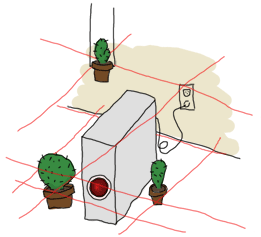
\includegraphics[width=1\linewidth]{cacti-laser.png}
\end{wrapfigure}
